\RequirePackage{luatex85}
\documentclass[tikz]{standalone}
\usepackage{pgfplots}
\pgfplotsset{compat=newest}
\pgfplotsset{every axis legend/.append style={%
cells={anchor=west}}
}
\usetikzlibrary{arrows}
\tikzset{>=stealth'}

\begin{document}
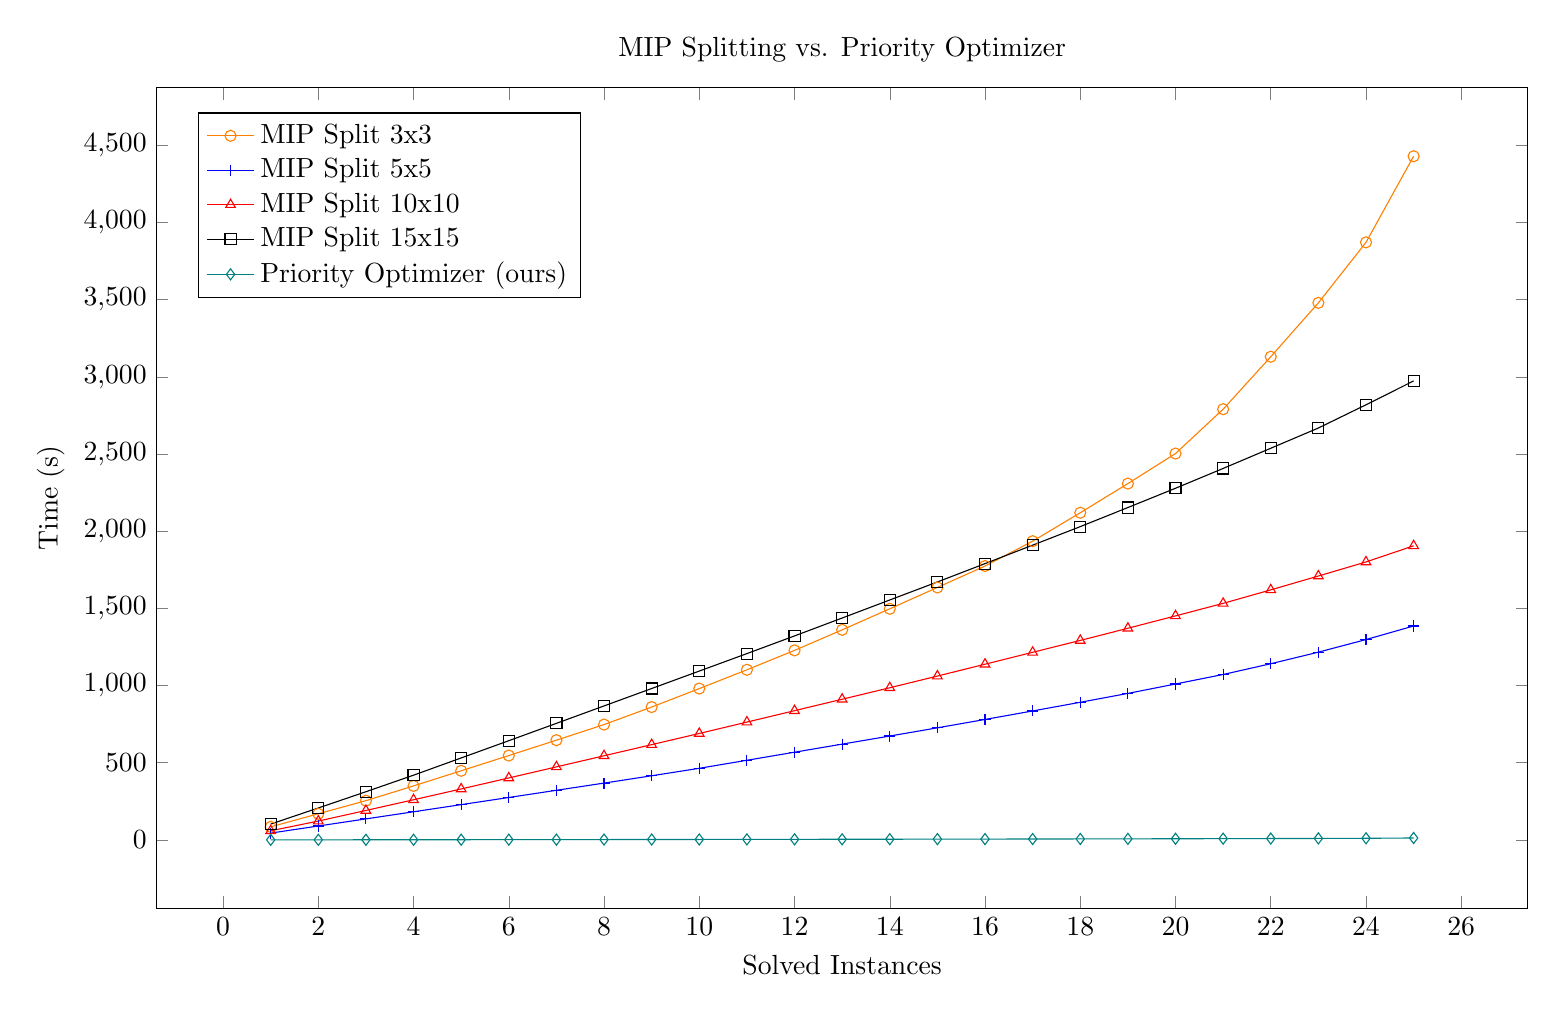
\begin{tikzpicture}[]
\begin{axis}[
  legend pos = {north west},
  ylabel = {Time (s)},
  title = {MIP Splitting vs. Priority Optimizer},
  xlabel = {Solved Instances},
  black, width=19cm, height=12cm
]

\addplot+[
  mark size = {2.0},
  mark=o, orange
] coordinates {
  (1.0, 84.471548824)
  (2.0, 169.184102295)
  (3.0, 254.286665976)
  (4.0, 349.817230062)
  (5.0, 447.762357258)
  (6.0, 546.562359169)
  (7.0, 646.178377296)
  (8.0, 747.220257638)
  (9.0, 860.7285290680001)
  (10.0, 980.4510845110001)
  (11.0, 1102.216732515)
  (12.0, 1227.805087577)
  (13.0, 1361.036248224)
  (14.0, 1497.3291332190001)
  (15.0, 1635.640750186)
  (16.0, 1774.596283672)
  (17.0, 1935.448221739)
  (18.0, 2119.714354179)
  (19.0, 2308.714006924)
  (20.0, 2503.283998973)
  (21.0, 2790.644134453)
  (22.0, 3130.639947745)
  (23.0, 3479.820086048)
  (24.0, 3871.722035719)
  (25.0, 4429.75267912)
};
\addlegendentry{{}{MIP Split 3x3}}

\addplot+[
  mark size = {2.0},
  mark=+, blue
] coordinates {
  (1.0, 44.119652564)
  (2.0, 90.007085069)
  (3.0, 136.074697651)
  (4.0, 182.184164469)
  (5.0, 228.473871975)
  (6.0, 274.816470052)
  (7.0, 321.407950188)
  (8.0, 368.02600204)
  (9.0, 415.485013955)
  (10.0, 463.920789672)
  (11.0, 515.888939964)
  (12.0, 568.182164616)
  (13.0, 620.5424410950001)
  (14.0, 672.956921658)
  (15.0, 726.1626423360001)
  (16.0, 780.389346656)
  (17.0, 835.478026952)
  (18.0, 891.677096781)
  (19.0, 949.152762597)
  (20.0, 1010.149598114)
  (21.0, 1071.79531676)
  (22.0, 1141.4749495740002)
  (23.0, 1216.4237920450003)
  (24.0, 1298.0613424290002)
  (25.0, 1385.9523678410003)
};
\addlegendentry{{}{MIP Split 5x5}}

\addplot+[
  mark size = {2.0},
  mark=triangle, red
] coordinates {
  (1.0, 59.066515686)
  (2.0, 122.04094498399999)
  (3.0, 190.691970747)
  (4.0, 259.98555180799997)
  (5.0, 330.096246959)
  (6.0, 401.334186723)
  (7.0, 473.135282494)
  (8.0, 545.068623087)
  (9.0, 617.201494361)
  (10.0, 689.58492099)
  (11.0, 763.291304044)
  (12.0, 837.235787891)
  (13.0, 911.4665053379999)
  (14.0, 985.7587810199999)
  (15.0, 1061.5373810429999)
  (16.0, 1138.412968833)
  (17.0, 1215.409279062)
  (18.0, 1292.437584153)
  (19.0, 1371.243080252)
  (20.0, 1451.439743745)
  (21.0, 1532.580995422)
  (22.0, 1619.938195384)
  (23.0, 1709.797294605)
  (24.0, 1800.949225652)
  (25.0, 1905.468135937)
};
\addlegendentry{{}{MIP Split 10x10}}

\addplot+[
  mark size = {2.0},
  mark=square, black
] coordinates {
  (1.0, 102.433696366)
  (2.0, 206.756899317)
  (3.0, 312.132791161)
  (4.0, 419.30182585299997)
  (5.0, 531.0086464579999)
  (6.0, 642.7492191299999)
  (7.0, 755.1885432209999)
  (8.0, 868.0160250499999)
  (9.0, 980.8932412879999)
  (10.0, 1093.9130246539999)
  (11.0, 1207.1386604159998)
  (12.0, 1321.6730144869998)
  (13.0, 1437.670402994)
  (14.0, 1554.5100809829999)
  (15.0, 1671.3738994439998)
  (16.0, 1790.1326972639997)
  (17.0, 1909.8237503019998)
  (18.0, 2029.7586405539998)
  (19.0, 2153.5468346949997)
  (20.0, 2278.3928570699995)
  (21.0, 2406.7897943719995)
  (22.0, 2537.5991667369995)
  (23.0, 2668.8083323239994)
  (24.0, 2819.3058008719995)
  (25.0, 2973.9098147599993)
};
\addlegendentry{{}{MIP Split 15x15}}

\addplot+[
  mark size = {2.0},
  mark=diamond,teal
] coordinates {
  (1.0, 0.199318859)
  (2.0, 0.431523422)
  (3.0, 0.675667996)
  (4.0, 0.948479469)
  (5.0, 1.239599299)
  (6.0, 1.546455781)
  (7.0, 1.854391283)
  (8.0, 2.177631634)
  (9.0, 2.531236597)
  (10.0, 2.898883621)
  (11.0, 3.268198786)
  (12.0, 3.649817)
  (13.0, 4.033394907)
  (14.0, 4.427159368)
  (15.0, 4.833887184)
  (16.0, 5.252577143)
  (17.0, 5.728226716)
  (18.0, 6.234611323)
  (19.0, 6.792864576)
  (20.0, 7.386304673000001)
  (21.0, 8.055118502000001)
  (22.0, 8.744375995)
  (23.0, 9.481529655000001)
  (24.0, 10.398286101)
  (25.0, 12.368083321)
};
\addlegendentry{{}{Priority Optimizer (ours)}}

\end{axis}
\end{tikzpicture}

\end{document}
